\documentclass[11pt]{article}

% Use [review] for the anonymised draft sent to the LLM TA Judge, [preprint] for the final report.
\usepackage[preprint]{acl}

\usepackage{times}
\usepackage{latexsym}
\usepackage[T1]{fontenc}
\usepackage[utf8]{inputenc}
\usepackage{microtype}
\usepackage{graphicx}
\usepackage{CJKutf8}
\newcommand{\zh}[1]{\begin{CJK}{UTF8}{bsmi}#1\end{CJK}}
\usepackage{booktabs}
\usepackage{amsmath}
\usepackage{amssymb}
\usepackage{tikz}
\usetikzlibrary{positioning,arrows.meta}

\graphicspath{{../figures/}}
\newcommand{\ours}{LvU}

\title{Money Laundering Is Not an Outlier: Detecting Illicit Bitcoin Transactions Without Illicit Labels}

\author{
  \textbf{Team G13} \\
  \zh{李尚哲} 314580057 \quad \zh{呂丞頤} 314580055 \quad \zh{黃駿甯} 314580075 \quad \zh{吳美真} 414551035 \\
  \zh{孫傅康} 112550176 \quad \zh{傅維雨} 112550149 \quad \zh{張凱華} 315554024 \quad \zh{李玠廷} 315554034 \\
  \url{https://github.com/leeshuncher/DataMiningHW2}
}

\begin{document}
\maketitle

\begin{abstract}
Compliance teams at cryptocurrency exchanges must flag laundering transactions, yet confirmed illicit labels are scarce and late, while licit counterparties are easy to label.
On the Elliptic Bitcoin graph (203,769 transactions, 49 time steps) we show that illicit transactions are \emph{not} outliers: only 1.7\% exceed a 3$\sigma$ rule versus 22.3\% of licit ones, so one-class detectors rank them \emph{below} normal (test ROC-AUC 0.17).
We therefore separate labeled licit from unlabeled transactions (\ours{}), a positive-unlabeled detector that never sees an illicit label during fitting.
On a chronological test split, \ours{} reaches PR-AUC 0.546\,$\pm$\,0.024 (8.4$\times$ prevalence) and 82\% precision in its top 100 alerts, recovering 69\% of supervised XGBoost's PR-AUC.
Ablations show that 1\% illicit contamination of the licit labels destroys this gain, and every method fails after a dark-market shutdown.
\end{abstract}

% ---------------------------------------------------------------------------
\section{Introduction}

\paragraph{Scenario and stakeholders.}
Virtual-asset service providers must screen the transactions they touch for money laundering.
Every alert goes to a compliance analyst, who decides whether to freeze funds and file a suspicious-activity report.
A missed laundering transaction (FN) exposes the provider to regulatory penalties; a false alert (FP) costs analyst time from a fixed weekly review budget.

\paragraph{Motivation.}
Supervised detectors work well on Bitcoin data \citep{weber2019aml} but need confirmed illicit labels, which take investigations and arrive late, whereas \emph{normal} labels are cheap (known exchanges and miners are tagged automatically).
One-class models trained on licit data, which treat anomalies as rare points far from normal data \citep{chandola2009survey}, look like the natural label-free choice, yet \citet{lorenz2020label} found that they perform poorly and that illicit instances are not actually outlying.
We quantify this failure, explain it, and turn the explanation into a detector.

\paragraph{Definition of anomaly.}
The unit of detection is one Bitcoin transaction (a graph node).
A transaction is anomalous if the Elliptic labels attribute it to an illicit entity (scams, malware, ransomware, Ponzi schemes, terrorist organisations); it is normal if attributed to a licit entity (exchanges, wallet providers, miners).
Example normal sample: tx 378120377 (step 16, licit; \texttt{local\_53}$=0.92$, in/out degree 0/2).
Example anomaly: tx 232014511 (step 1, illicit; \texttt{local\_53}$=-0.49$, degree 1/1).

\paragraph{Research question.}
\emph{Can a detector fitted without any illicit label rank illicit Bitcoin transactions above licit ones on future time steps, even though illicit transactions are not outliers?}

\paragraph{Contributions.}
(C1) We show that illicit transactions are less extreme than licit ones (1.7\% vs.\ 22.3\% beyond 3$\sigma$), which inverts one-class detectors to ROC-AUC 0.17--0.20 (\S\ref{sec:eda}, \S\ref{sec:results}).
(C2) A licit-vs-unlabeled (\ours{}) detector reaches test PR-AUC 0.546 and P@100 0.82 without illicit labels, significantly above label-free baselines and below supervised ones (\S\ref{sec:results}).
(C3) It is robust to the unlabeled pool size but collapses when 1\% of licit labels are wrong (\S\ref{sec:ablation}).
(C4) 42\% of its misses fall after a dark-market shutdown, a blind spot shared with supervised models (\S\ref{sec:analysis}).

% ---------------------------------------------------------------------------
\section{Related Work}

\paragraph{Data category and literature.}
Our data are a \emph{graph}: transactions are nodes and payment flows are directed edges, so each node has relational context.
\citet{weber2019aml} released the Elliptic data set and compared supervised models on a 70:30 temporal split (Table~\ref{tab:related}); Random Forest on all features gave the best illicit F1 (0.788), ahead of graph convolutional networks.
EvolveGCN \citep{pareja2020evolvegcn} models the graph sequence over time and reports that no model recovers after the dark-market shutdown.
\citet{lorenz2020label} found that seven unsupervised detectors reach illicit F1 of at most 0.19 (LOF), and proposed active learning, which matches a supervised baseline with 5\% of the labels.
Positive-unlabeled (PU) learning trains a classifier from one labeled class plus unlabeled data \citep{elkan2008pu,bekker2020pu}; Deep SAD \citep{ruff2020deepsad} instead uses a few labeled anomalies.

\begin{table}[t]
\centering\small
\setlength{\tabcolsep}{3pt}
\begin{tabular}{@{}llll@{}}
\toprule
Work & Paradigm & Method & Ill.\ F1 \\
\midrule
\citet{weber2019aml} & supervised & RF, AF & 0.788 \\
\citet{weber2019aml} & supervised & GCN & 0.628 \\
\citet{lorenz2020label} & unsupervised & LOF (best) & $\le$0.19 \\
\citet{lorenz2020label} & unsupervised & IF & $\le$0.01 \\
\midrule
Ours & PU, no ill.\ labels & \ours{} & 0.398 \\
Ours & supervised (T3a) & RF, AF & 0.541 \\
\bottomrule
\end{tabular}
\caption{Prior results on Elliptic (illicit-class F1). Prior work trains on steps 1--34; we train on 1--29 and tune $\tau$ on 30--34, so numbers give context, not a direct comparison.}
\label{tab:related}
\end{table}

\paragraph{Positioning and method selection.}
Tier~1 assumes anomalies are extreme in some feature (3$\sigma$ rule) or nothing at all (random score).
Tier~2 assumes illicit mass is over-represented in unlabeled relative to licit data (our \ours{}); we also report the one-class Isolation Forest \citep{liu2008iforest}, which assumes anomalies are easy to isolate.
Tier~3 uses full supervision: Random Forest \citep{breiman2001rf} as in \citet{weber2019aml}, and XGBoost \citep{chen2016xgboost}.
Unlike prior work, we fit without illicit labels, explain \emph{why} outlier detectors invert, and analyse failures per transaction.

% ---------------------------------------------------------------------------
\section{Task Definition and Data}
\label{sec:data}

\paragraph{Data set.}
We use the Elliptic Data Set \citep{weber2019aml}, obtained from the official Kaggle release (license CC BY-NC-ND 4.0); our repository downloads and checksums it.
It contains $N=203{,}769$ transactions and 234,355 edges in 49 time steps about two weeks apart; edges never cross time steps.
Each node has $D=166$ anonymised features: the time step, 93 local features (LF; e.g.\ fees, input/output counts and volumes) and 72 aggregates over one-hop neighbours (AF).
We add in/out degree from the edge list.

\paragraph{Labels.}
Ground truth comes from a heuristics-based labelling of the entities behind each transaction \citep{weber2019aml}: 4,545 illicit, 42,019 licit, and 157,205 \emph{unknown}.
Labels may be noisy (heuristic, entity-level attribution), and unknown transactions contain both classes; they are never evaluated, but \ours{} uses them as unlabeled training data.
The paradigm is semi-supervised: licit labels and unlabeled data for fitting, illicit labels only for validation-based selection.

\begin{table}[t]
\centering\small
\setlength{\tabcolsep}{3pt}
\begin{tabular}{@{}lrrrrrr@{}}
\toprule
Split & Steps & Tx & Licit & Illicit & Unknown & Ill./lab. \\
\midrule
train & 1--29 & 120,804 & 23,510 & 2,871 & 94,423 & 10.9\% \\
val & 30--34 & 15,461 & 2,922 & 591 & 11,948 & 16.8\% \\
test & 35--49 & 67,504 & 15,587 & 1,083 & 50,834 & 6.5\% \\
\midrule
all & 1--49 & 203,769 & 42,019 & 4,545 & 157,205 & 9.8\% \\
\bottomrule
\end{tabular}

\caption{Chronological split shared by all methods.}
\label{tab:data}
\end{table}

\paragraph{Class imbalance.}
Overall, 2.2\% of transactions are illicit; among labeled ones the ratio is 9.8\% vs.\ 90.2\% (1\,:\,9.2), and on the test split 6.5\% (1\,:\,14.4).
A model that predicts ``always licit'' reaches 93.5\% test accuracy with zero recall, so we never report accuracy.
We use threshold-free ranking metrics (PR-AUC) and choose $\tau$ to maximise F1 rather than relying on a 0.5 cut-off.

% ---------------------------------------------------------------------------
\section{Exploratory Feature Analysis}
\label{sec:eda}

All statistics use the training split only (Figure~\ref{fig:eda}).

\begin{figure*}[t]
\centering
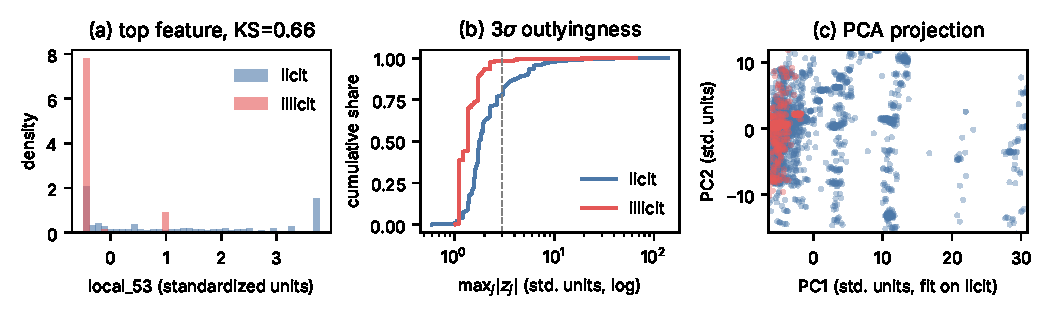
\includegraphics[width=\textwidth]{eda.pdf}
\caption{Training split only. (a) The most separating feature: illicit transactions concentrate on one value. (b) Cumulative share of the largest $|z|$-score (w.r.t.\ licit statistics): illicit transactions are \emph{less} extreme than licit ones; dashed line = 3$\sigma$. (c) PCA fitted on licit data: illicit points form a compact cluster inside the region occupied by licit ones.}
\label{fig:eda}
\end{figure*}

\paragraph{Distribution contrast.}
Figure~\ref{fig:eda}a shows \texttt{local\_53}, the feature with the largest Kolmogorov--Smirnov (KS) distance between classes (0.66, mutual information 0.21 nats).
Most illicit transactions sit on a single value ($-0.49$, shared by 83\% of illicit but 18\% of licit training transactions), whereas licit values spread over the whole range.
Figure~\ref{fig:eda}b is the key observation: only 1.7\% of illicit transactions have any local feature beyond 3$\sigma$ of the licit distribution, against 22.3\% of licit transactions.
In PCA space (Figure~\ref{fig:eda}c), illicit points occupy one compact region; licit points scatter over many clusters.

\paragraph{Separability and redundancy.}
Local features separate the classes better than neighbour aggregates (mean KS 0.38 vs.\ 0.27; 63 vs.\ 30 features with KS $>0.3$; mean MI 0.088 vs.\ 0.060 nats) and degree (0.20).
89 feature pairs have $|r|>0.95$, and licit behaviour drifts moderately within training (mean KS 0.11, steps 1--14 vs.\ 15--29).

\paragraph{Hypotheses.}
\textbf{H1}: Outlier-based scores (3$\sigma$, Isolation Forest, Mahalanobis) will rank illicit transactions \emph{below} licit ones.
\textbf{H2}: A model that contrasts licit data with unlabeled data will rank them above, because the compact illicit mode is denser in the unlabeled pool than among labeled licit transactions.
\textbf{H3}: Neighbour aggregates and degree will add little to local features.
We test H1--H2 in \S\ref{sec:results}--\ref{sec:ablation} and H3 in \S\ref{sec:ablation}.

% ---------------------------------------------------------------------------
\section{Method}
\label{sec:method}

\begin{figure}[t]
\centering
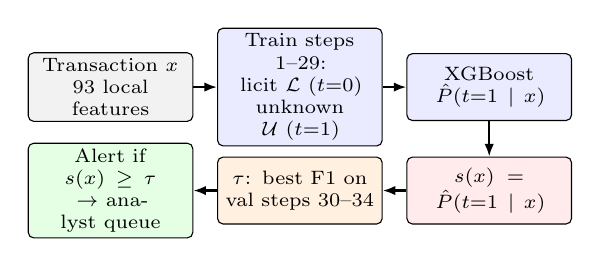
\begin{tikzpicture}[
  box/.style={draw, rounded corners=2pt, align=center, font=\scriptsize, minimum height=0.85cm, inner sep=2pt, text width=1.95cm},
  arr/.style={-{Latex[length=1.6mm]}, thick}]
\node[box, fill=gray!10] (x) {Transaction $x$\\93 local features};
\node[box, fill=blue!8, right=0.3cm of x] (tr) {Train steps 1--29:\\licit $\mathcal{L}$ ($t{=}0$)\\unknown $\mathcal{U}$ ($t{=}1$)};
\node[box, fill=blue!8, right=0.3cm of tr] (m) {XGBoost\\$\hat{P}(t{=}1 \mid x)$};
\node[box, fill=red!8, below=0.45cm of m] (s) {$s(x)=\hat{P}(t{=}1\mid x)$};
\node[box, fill=orange!12, left=0.3cm of s] (tau) {$\tau$: best F1 on\\val steps 30--34};
\node[box, fill=green!10, left=0.3cm of tau] (a) {Alert if $s(x)\ge\tau$\\$\rightarrow$ analyst queue};
\draw[arr] (x) -- (tr);
\draw[arr] (tr) -- (m);
\draw[arr] (m) -- (s);
\draw[arr] (s) -- (tau);
\draw[arr] (tau) -- (a);
\end{tikzpicture}
\caption{\ours{} pipeline. No illicit label is used for fitting; labeled illicit transactions of the validation steps only set $\tau$.}
\label{fig:pipeline}
\end{figure}

\paragraph{Pipeline.}
Figure~\ref{fig:pipeline} shows the Tier~2 pipeline.
The input is the 93 local features of a transaction, used as released (already scaled); the time step is dropped so that the model cannot memorise periods.
We build a training set from the training steps: every labeled licit transaction gets target $t=0$ and every unknown transaction gets $t=1$ (23,510 vs.\ 94,423 rows).
Illicit training transactions are \emph{not} used.
An XGBoost classifier (300 trees, depth 6, learning rate 0.1, row/column subsampling 0.8) learns $\hat{P}(t{=}1\mid x)$.

\paragraph{Anomaly score.}
The score is $s(x)=\hat{P}(t{=}1\mid x)$.
For a well-calibrated classifier, $s$ is monotone in the density ratio $p_{\mathcal{U}}(x)/p_{\mathcal{L}}(x)$.
If the unknown pool is a mixture $p_{\mathcal{U}}=\pi\,p_{\text{ill}}+(1-\pi)\,p_{\text{lic}}$ and labeled licit data follow $p_{\text{lic}}$, the ratio equals $(1-\pi)+\pi\,p_{\text{ill}}(x)/p_{\text{lic}}(x)$ and therefore ranks transactions exactly by how much more likely they are under the illicit than the licit distribution \citep{elkan2008pu}.
Unlike an outlier score, this ranking rewards a dense illicit mode that licit data rarely reach (H2).

\paragraph{Threshold and error costs.}
$\tau$ is the score that maximises F1 on the labeled transactions of validation steps 30--34; the test split is never used.
An FN lets laundered funds pass (regulatory risk); an FP costs analyst minutes.
Because an FN is costlier, we accept the recall-leaning $\tau$ that F1 selects: about 2.5 false alerts per caught transaction at 65\% recall (alternatives in \S\ref{sec:ablation}).

% ---------------------------------------------------------------------------
\section{Experimental Setup}
\label{sec:setup}

\paragraph{Split and leakage prevention.}
All methods share one chronological split by time step (Table~\ref{tab:data}): train 1--29, validation 30--34, test 35--49.
The train+validation/test boundary is the 70:30 split of \citet{weber2019aml}.
One-class models fit licit training rows only; \ours{} fits licit and unknown training rows; supervised models fit labeled training rows.
Scalers (3$\sigma$, LOF, $k$NN) are fit on licit training rows; the test set is scored once per seed.

\paragraph{Configurations.}
\ours{} hyperparameters were chosen by validation PR-AUC over feature set $\in$\{LF, AF, AF+degree\}, depth $\in\{4,6,8\}$ and trees $\in\{100,300\}$ (best: LF, 6, 300; validation PR-AUC 0.901).
Isolation Forest uses 200 trees with \texttt{max\_samples} $\in\{256,2048\}$ (best: 2048, LF).
Random Forest follows \citet{weber2019aml} (50 trees, 50 features per split, AF); XGBoost uses the same settings as \ours{} on AF.
Every stochastic method runs with 5 seeds.
Software: Python 3.13, scikit-learn 1.9 \citep{pedregosa2011sklearn}, XGBoost 3.4; hardware: 4 vCPUs, 16\,GB RAM, no GPU.

\paragraph{Metrics.}
(1) \textbf{PR-AUC} (average precision) is our primary metric: it ignores the large number of easy true negatives and is informative under imbalance \citep{saito2015prc}; its random baseline equals the prevalence.
(2) \textbf{P@100}, the precision of the 100 highest-scored test transactions, models a fixed analyst budget.
(3) \textbf{F1@$\tau$} evaluates the deployed decision.
ROC-AUC is reported to show inversion ($<0.5$).

% ---------------------------------------------------------------------------
\section{Results}
\label{sec:results}

\begin{table*}[t]
\centering\small
\setlength{\tabcolsep}{2.6pt}
\begin{tabular}{@{}llcccccccc@{}}
\toprule
 & & & & & & \multicolumn{2}{c}{PR-AUC by period} & Fit & Score \\
\cmidrule(lr){7-8}
Tier & Method & PR-AUC & ROC-AUC & F1@$\tau$ & P@100 & steps 35--42 & 43--49 & (s) & ($\mu$s/tx) \\
\midrule
T1a & Random score & 0.065$\pm$0.001 & 0.495$\pm$0.006 & 0.122$\pm$0.000 & 0.060$\pm$0.017 & 0.091 & 0.027 & 0.1 & 0.0 \\
T1b & 3$\sigma$ rule (max $|z|$) & 0.053 & 0.326 & 0.010 & 0.040 & 0.075 & 0.028 & 0.1 & 0.2 \\
\midrule
T2$'$ & One-class Isolation Forest & 0.038$\pm$0.000 & 0.170$\pm$0.008 & 0.121$\pm$0.002 & 0.000 & 0.053 & 0.021 & 0.7 & 11.9 \\
T2 & \textbf{LvU classifier (ours)} & 0.546$\pm$0.024 & 0.865$\pm$0.002 & 0.398$\pm$0.011 & 0.822$\pm$0.020 & 0.743 & 0.025 & 4.6 & 1.5 \\
\midrule
T3a & Random Forest (sup.) & 0.767$\pm$0.003 & 0.891$\pm$0.004 & 0.541$\pm$0.138 & \textbf{1.000} & 0.897 & 0.028 & 5.7 & 2.2 \\
T3b & XGBoost (sup.) & \textbf{0.790$\pm$0.001} & \textbf{0.922$\pm$0.002} & \textbf{0.675$\pm$0.056} & \textbf{1.000} & \textbf{0.914} & 0.036 & 2.8 & 1.7 \\
\multicolumn{2}{l}{\emph{prevalence (= random PR-AUC)}} & 0.065 & & & & 0.092 & 0.025 & & \\
\bottomrule
\end{tabular}

\caption{Test results (labeled transactions of steps 35--49), mean\,$\pm$\,std over 5 seeds (deterministic methods: one run). F1 uses $\tau$ tuned on validation (3$\sigma$ rule: $\tau=3$). Best per column in bold. Period columns split the test set at the dark-market shutdown (step 43).}
\label{tab:main}
\end{table*}

\paragraph{Main comparison.}
Table~\ref{tab:main} supports H1: the 3$\sigma$ rule and the one-class Isolation Forest rank illicit transactions below licit ones (ROC-AUC 0.33 and 0.17) and fall under the random baseline in PR-AUC.
Their val-tuned $\tau$ degenerates to ``alert on everything'' (F1 0.12, as for random scores).
\ours{} supports H2: PR-AUC rises to 0.546\,$\pm$\,0.024 (8.4$\times$ prevalence) and 82\% of its top-100 alerts are illicit.
The gap to the best label-free baseline (T1a) is significant (paired $t$-test over seeds, $p<10^{-5}$; bootstrap 95\% CI of the PR-AUC gap [0.450, 0.513]).

\paragraph{Against Tier 3.}
Supervised models remain clearly better: XGBoost reaches PR-AUC 0.790 and RF 0.767; the gaps to \ours{} are significant (bootstrap CI vs.\ XGBoost [$-$0.268, $-$0.218], $p<10^{-4}$).
\ours{} recovers 69\% of XGBoost's PR-AUC without a single illicit label.
It loses because it learns ``unlabeled-like'' rather than ``illicit'': licit transactions resembling the unlabeled mass also score high (\S\ref{sec:analysis}).
RF's F1 varies across seeds (0.42--0.80) while its PR-AUC does not: a $\tau$ tuned on validation steps with 16.8\% prevalence transfers poorly to a 6.5\% test period.
All models train in under 6\,s and score in 1--12\,$\mu$s per transaction, so cost does not separate them.

\subsection{Controlled Ablations}
\label{sec:ablation}

\begin{table}[t]
\centering\small
\setlength{\tabcolsep}{3pt}
\begin{tabular}{@{}lccc@{}}
\toprule
Setting & Test PR-AUC & $\Delta$ & Val \\
\midrule
\multicolumn{4}{@{}l}{\emph{A1: illicit rows hidden in licit side}} \\
\quad 0\% (ours) & 0.546$\pm$0.024 & --- & 0.871 \\
\quad 1\% & 0.142$\pm$0.007 & $-0.404$ & 0.359 \\
\quad 5\% & 0.098$\pm$0.003 & $-0.448$ & 0.247 \\
\quad 10\% & 0.091$\pm$0.004 & $-0.455$ & 0.217 \\
\multicolumn{4}{@{}l}{\emph{A2: fraction of unlabeled pool used}} \\
\quad 5\% & 0.546$\pm$0.018 & $+0.000$ & 0.849 \\
\quad 25\% & 0.520$\pm$0.047 & $-0.026$ & 0.863 \\
\quad 50\% & 0.551$\pm$0.040 & $+0.005$ & 0.833 \\
\quad 100\% (ours) & 0.546$\pm$0.024 & --- & 0.871 \\
\multicolumn{4}{@{}l}{\emph{A3: label-free scoring function}} \\
\quad one-class IF & 0.037$\pm$0.000 & $-0.509$ & 0.108 \\
\quad one-class Mahalanobis & 0.038$\pm$0.001$^\dagger$ & $-0.508$ & 0.097 \\
\quad one-class LOF & 0.190$\pm$0.010$^\dagger$ & $-0.356$ & 0.218 \\
\quad PU $k$NN ratio & 0.194$\pm$0.010$^\dagger$ & $-0.352$ & 0.713 \\
\quad PU classifier (ours) & 0.546$\pm$0.024 & --- & 0.871 \\
\multicolumn{4}{@{}l}{\emph{A4: feature set}} \\
\quad LF, 93 local (ours) & 0.546$\pm$0.024 & --- & 0.871 \\
\quad AF (+72 aggregates) & 0.557$\pm$0.037 & $+0.011$ & 0.768 \\
\quad AF + in/out degree & 0.509$\pm$0.043 & $-0.037$ & 0.756 \\
\quad AF + 2-hop aggregates & 0.536$\pm$0.046 & $-0.010$ & 0.783 \\
\bottomrule
\end{tabular}

\caption{Ablations of \ours{} on the test split, one factor at a time (5 seeds unless deterministic; F1: mean). $\Delta$ = PR-AUC change vs.\ the full method.}
\label{tab:ablation}
\end{table}

\paragraph{A1: contamination of the normal labels (AD-specific).}
Replacing just 1\% of the licit training rows with illicit ones (235 rows) cuts PR-AUC from 0.546 to 0.142, far beyond the seed std.
Because illicit transactions form one compact mode, a few hundred of them labeled $t=0$ suffice to tell the classifier that this mode is ``licit''.
This is an honest negative result: \ours{} needs clean licit labels.

\paragraph{A2: size of the unlabeled pool (AD-specific).}
Using 5\% of the unknown pool (4.7k rows) gives the same PR-AUC (0.546); all differences are within one std, so a small unlabeled sample already contains the illicit mode.

\paragraph{A3: scoring function (AD-specific).}
Holding features and data fixed, outlier scores invert (Isolation Forest 0.037, Mahalanobis with Ledoit--Wolf shrinkage \citep{ledoit2004shrinkage} 0.038).
Local density scores, LOF \citep{breunig2000lof} and a $k$NN density ratio between licit and unlabeled data, recover some signal (0.19).
The classifier-based density ratio is best (0.546).

\paragraph{A4: graph features.}
Adding the 72 neighbour aggregates changes PR-AUC by $+$0.011 and adding degree by $-$0.037, both within about one seed std; this supports H3.
AF raises recall but lowers F1, because the validation threshold transfers worse.

\paragraph{Threshold strategy.}
For the same scores (Table~\ref{tab:threshold}), the label-free 95th-percentile rule doubles the alerts (F1 0.27); a budget of 30 alerts per step gives the highest precision (0.48) at 20\% recall.

\begin{table}[t]
\centering\small
\setlength{\tabcolsep}{3pt}
\begin{tabular}{@{}lcccc@{}}
\toprule
$\tau$ rule & Alerts & Precision & Recall & F1 \\
\midrule
best F1 on val (ours) & 2459 & 0.288 & 0.650 & 0.398 \\
95th pct.\ licit train & 5420 & 0.159 & 0.797 & 0.266 \\
top-30 per time step & 450 & 0.484 & 0.201 & 0.284 \\
\bottomrule
\end{tabular}

\caption{Alert rules for \ours{} on the test split (15 steps); mean of 5 seeds, std $\le$0.04.}
\label{tab:threshold}
\end{table}

% ---------------------------------------------------------------------------
\section{Analysis}
\label{sec:analysis}

\begin{figure}[t]
\centering
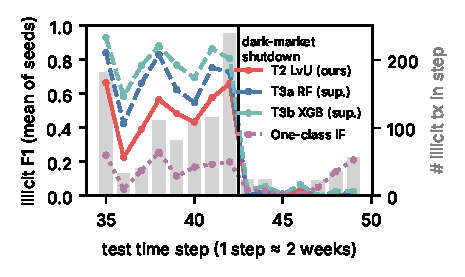
\includegraphics[width=\columnwidth]{per_step.pdf}
\caption{Illicit F1 per test step (lines, left axis) and number of illicit transactions (bars, right axis). Every method collapses after the dark-market shutdown at step 43. The one-class IF rises only because it alerts on everything.}
\label{fig:perstep}
\end{figure}

\paragraph{Temporal failure.}
Figure~\ref{fig:perstep} reproduces the observation of \citet{weber2019aml}: after a dark market closes at step 43, every model fails.
\ours{}'s F1 drops from 0.50 (steps 35--42) to 0.01 (43--49), and its PR-AUC from 0.743 to 0.025, which equals the prevalence (Table~\ref{tab:main}).
Only 15.6\% of test illicit transactions fall in steps 43--49, but they account for 42\% of the misses of \ours{}.
Of the 398 misses (seed 0, $\tau=0.970$), 69\% are also missed by supervised RF: the blind spot lies in the data, not in our label-free setting.

\begin{table*}[t]
\centering\small
\begin{tabular}{@{}clrrcccl@{}}
\toprule
\# & Type & txId & Step & $s(x)$ & Top-SHAP feature & RF & Likely cause \\
\midrule
1 & FN & 97069571 & 40 & 0.014 & local\_48$=0.09$ & 0.04 & licit-typical profile \\
2 & FN & 73003591 & 42 & 0.970 & local\_53$=-0.49$ & 0.76 & 73/93 features equal \#4 \\
3 & FP & 169360875 & 45 & 1.000 & local\_53$=-0.49$ & 0.03 & licit tx in illicit mode \\
4 & FP & 73160604 & 42 & 0.970 & local\_53$=-0.49$ & 0.41 & 73/93 features equal \#2 \\
\bottomrule
\end{tabular}

\caption{Failure cases of \ours{} (seed 0, $\tau=0.970$). RF = supervised Random Forest score (mean of seeds; its mean $\tau\approx0.37$). Top-SHAP = local feature with the largest attribution for this transaction.}
\label{tab:cases}
\end{table*}

\paragraph{Failure cases.}
Table~\ref{tab:cases} lists four test errors.
\#1 is a complete inversion: an illicit transaction with $s=0.014$ whose \texttt{local\_53}$=1.81$ lies above 99.6\% of illicit but at the 63rd percentile of licit training transactions; RF misses it too (0.04).
Cases \#2 (FN) and \#4 (FP) receive the identical score 0.970, just at $\tau$.
They share 73 of 93 local features (L2 distance 4.1 vs.\ a median of 10.2 to licit transactions), yet carry opposite labels.
No threshold can separate them; this points to label noise or to entities that reuse the same wallet software.
\#3 is a confident FP ($s=1.000$): a licit transaction sitting on the illicit mode \texttt{local\_53}$=-0.49$, which RF correctly scores 0.03.
Without illicit labels, \ours{} cannot learn which parts of the unlabeled mass are illicit.
\textbf{Shared pattern}: errors come from overlapping modes and post-shutdown drift, not model capacity; the first fix we would try is a few analyst-confirmed labels from the new period (active learning, \citealp{lorenz2020label}), not a larger model.

\begin{figure*}[t]
\centering
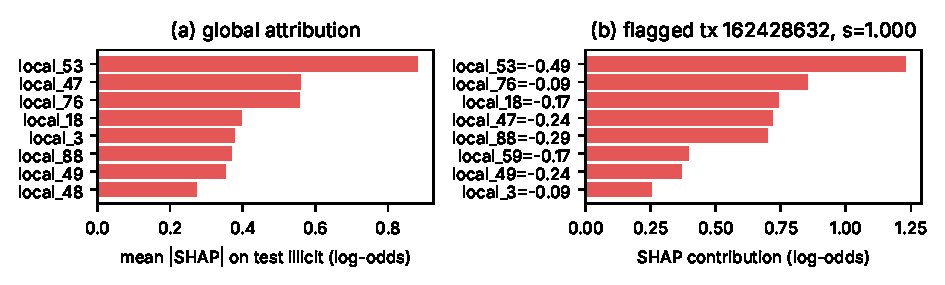
\includegraphics[width=0.85\textwidth]{shap.pdf}
\caption{TreeSHAP attributions of \ours{} (seed 0) in log-odds of $t=1$. (a) Mean $|$SHAP$|$ over test illicit transactions. (b) The highest-scored true positive: its value on the illicit mode \texttt{local\_53}$=-0.49$ contributes most.}
\label{fig:shap}
\end{figure*}

\paragraph{Interpretability.}
We explain \ours{} with exact TreeSHAP \citep{lundberg2020treeshap} (Figure~\ref{fig:shap}).
Globally, \texttt{local\_53}, \texttt{local\_47} and \texttt{local\_76} dominate; \texttt{local\_53} is also the top EDA feature, so the model uses the illicit mode found in \S\ref{sec:eda}.
For the flagged tx 162428632 ($s=1.000$; RF agrees, 0.94), \texttt{local\_53}$=-0.49$ adds 1.23 log-odds and five further local features each add 0.4--0.9.
An analyst would see that the transaction matches a pattern common in illicit flows, a reason to review but not proof; anonymised features limit trust until their meaning is disclosed.

\paragraph{Practical impact.}
At the validation threshold, \ours{} raises 2,459 alerts over 15 steps (about 164 per two-week step) and catches 65\% (about 704) of the 1,083 illicit test transactions; 71\% of its alerts are false.
With a budget of 30 alerts per step, 48\% of alerts are illicit, 7.4$\times$ the yield of random review.
Supervised RF catches ${\approx}$100 more with fewer alerts; \ours{} is a cold-start triage tool for providers without confirmed illicit cases.

% ---------------------------------------------------------------------------
\section{Conclusion and Limitations}

\paragraph{Key findings.}
Yes, with qualifications.
A detector fitted only on licit and unlabeled transactions ranks illicit Bitcoin transactions far above chance on future steps (PR-AUC 0.546 vs.\ 0.065; P@100 0.82), whereas outlier detectors invert (ROC-AUC 0.17), because illicit transactions form a compact, non-extreme mode.
It reaches 69\% of supervised PR-AUC, but it fails after the dark-market shutdown, like every model we tested.

\paragraph{Reflection and future work.}
The decision that mattered most was testing outlyingness in EDA (Figure~\ref{fig:eda}b); starting again, we would do it before implementing any one-class model.
Next steps: (i) query analyst labels for the highest-scoring unlabeled transactions after a drift alarm, to address the post-shutdown misses; (ii) estimate the class prior $\pi$ of the unlabeled pool \citep{bekker2020pu} to calibrate $\tau$ across periods.

\paragraph{Limitations.}
\emph{Data coverage}: one blockchain and 49 two-week steps (undisclosed calendar dates), with entity-level heuristic labels and anonymised features; 77\% of transactions are unlabeled, so all scores refer to labeled ones only.
\emph{Assumptions}: \ours{} assumes clean licit labels (A1 shows 1\% noise is fatal) and that the unlabeled pool contains the illicit modes of the future, which fails after the shutdown.
\emph{Generalisation}: the outlier inversion may not hold for fraud types that are genuinely extreme (e.g.\ large one-off thefts).

\paragraph{Deployment considerations.}
\emph{Concept drift}: illicit behaviour changed abruptly at step 43; retrain every few steps and monitor with a small labeled audit sample, since scores alone do not reveal a collapse.
\emph{Latency and privacy}: scoring takes ${\approx}1.5\,\mu$s per transaction, far below block times; blockchain data are public, but linking addresses to people falls under data-protection and AML rules.

% ---------------------------------------------------------------------------
\section*{Contributions of Each Member}

\begin{itemize}\setlength\itemsep{0pt}
\item \zh{李尚哲} (314580057): baselines (\S6).
\item \zh{呂丞頤} (314580055): data pipeline (\S3).
\item \zh{黃駿甯} (314580075): error analysis (\S8).
\item \zh{吳美真} (414551035): related work (\S1, 2, 9).
\item \zh{孫傅康} (112550176): EDA (\S4).
\item \zh{傅維雨} (112550149): ablations (\S7.1).
\item \zh{張凱華} (315554024): \ours{} method (\S5).
\item \zh{李玠廷} (315554034): main results (\S7).
\end{itemize}
All members: slides, conclusions, proofreading.

\paragraph{AI usage statement.}
We used Claude Code for code and drafting; the team chose the question and verified every number and citation.

\bibliography{refs}

\end{document}
